%! Author = Philipp Emmenegger
%! Date = 08/06/2021

\section{Project Planning}
\subsection{Rational Unified Process (RUP)}
Very comprehensive process (phases, disciplines, artifacts, roles)\\
Too heavy weighted for many projects
\subsubsection{Phases}
\textbf{Inception}
\begin{itemize}
    \item Appriximate vision
    \item Defining the scope
    \item Rough estimates for efforts
\end{itemize}
\textbf{Elaboration}
\begin{itemize}
    \item Identification of most requirements
    \item Iterative implementation of core architecture
    \item Resolution of high risks
    \item More realistic estimates for efforts
\end{itemize}
\textbf{Construction}
\begin{itemize}
    \item Iterative implementation of functionality
    \item Resolution of lower risks
    \item Preparation for deployment
\end{itemize}
\textbf{Transition}
\begin{itemize}
    \item Beta tests
    \item Deployment
    \item tie up any loose ends
\end{itemize}

\subsection{Scrum}
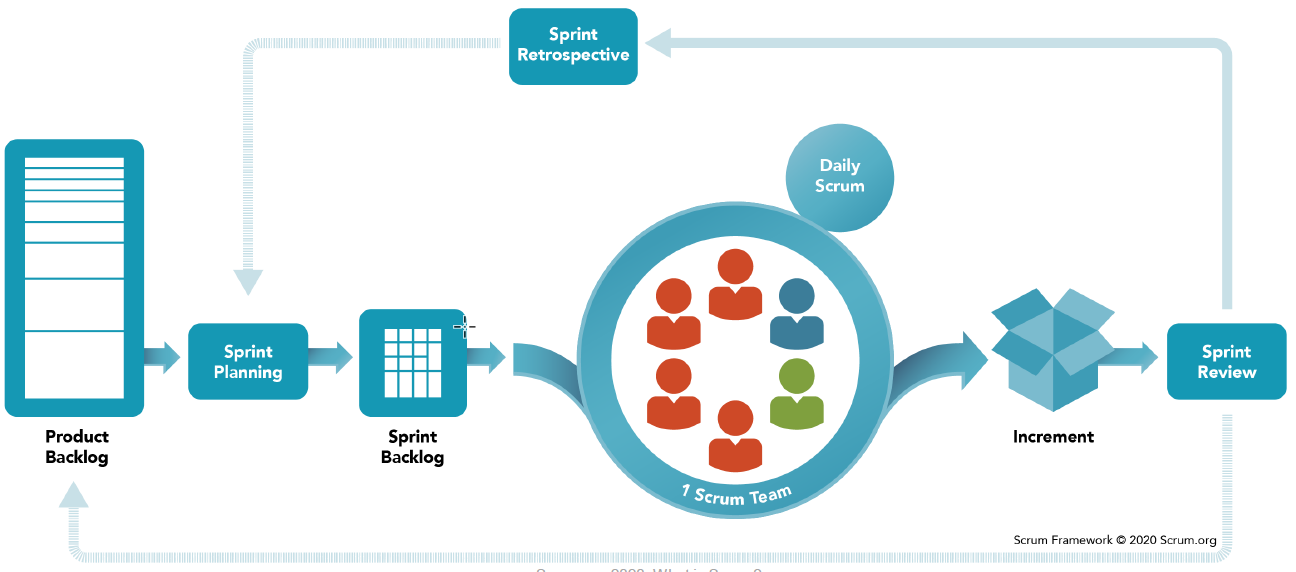
\includegraphics[width=\linewidth]{../img/scrum_overview.png}
\subsection{Combining RUP and Scrum}
\begin{itemize}
    \item Long-term planning and disciplines from RUP
    \item Short-term planning in iterations from Scrum
    \item Known as Scrum+
\end{itemize}
\subsubsection{Planning on different levels}
\textbf{Long-term}
\begin{itemize}
    \item Rough scopes \& estimates
    \item epics, brief use cases, etc.
\end{itemize}
\textbf{Short-Term}
\begin{itemize}
    \item Detailed scopes \& estimates
    \item user stories, tasks, etc.
\end{itemize}

\subsubsection{Work Items}
Everything you invest time should be tracked as a work item
\textbf{Sources:}
\begin{itemize}
    \item Functional Requirements
    \item Non-functional requirements
    \item Bugs
    \item Refactoring
    \item Knowledge acquisition
\end{itemize}
\textbf{Best Practices}
\begin{itemize}
    \item Created during Sprint planning
    \item Tracked in a tool
    \item Accessible by everyone
    \item Should be categorized for easier filtering and reporting
    \item Small enough to be done by a single person
    \item Should follow a workflow with different states
    \item As specific as possible, describe concrete tasks
\end{itemize}

\subsubsection{Documentation}
\textbf{What should be written down?}
\begin{itemize}
    \item Whatever is worth to be written down
    \item (Requirements, Software Architecture, Project planning, Project Tracking...)
\end{itemize}
\textbf{How should be documented?}
\begin{itemize}
    \item Focus on long-living, stable contents
    \item Use pictures
    \item Use generators where appropriate
    \item Prefer tools / formats which can be versioned
    \item Export documents on every milestone
\end{itemize}